\section{Implementation} \label{chapter:IMPLEMENTATION}

This chapter describes our implementation of object-versioning using ECMAScript 6 proxies\footnote{\url{http://wiki.ecmascript.org/doku.php?id=harmony:direct_proxies}, accessed February 3rd, 2014} in the Lively Kernel.
It presents the proxy's behavior and shows how proxies are inserted for ordinary references using source transformations.
The chapter also presents workarounds for the current state of ECMAScript 6 proxies and current limitations of using them.

\subsection{Using ECMAScript 6 Proxies for Object Versioning} \label{subsec:IMPLEMENTATION:1.2}

The ECMAScript 6 proxies \emph{stand in} for their target objects and intercept different interactions using \emph{traps}.
The implementation of the traps is provided by a separate \emph{handler} object.
When a proxy's handler does not implement a trap, the proxy forwards the intercepted interaction to the target.
On the hand, if all traps are implemented, all interaction can be handled without forwarding to the target object.

In our implementation, proxies delegate to one of multiple versions of an object.
In \autoref{fig:VersioningProxy} a proxy stands in for two versions of an \lstinline{address} object: The proxy's handler holds a reference to a \lstinline{versions} object, which in turn refers to the versions of the \lstinline{address} object.
The proxy's target is ommited from \autoref{fig:VersioningProxy} as we used the proxies as purely virtual objects.

\begin{figure}[h]
    \centering
    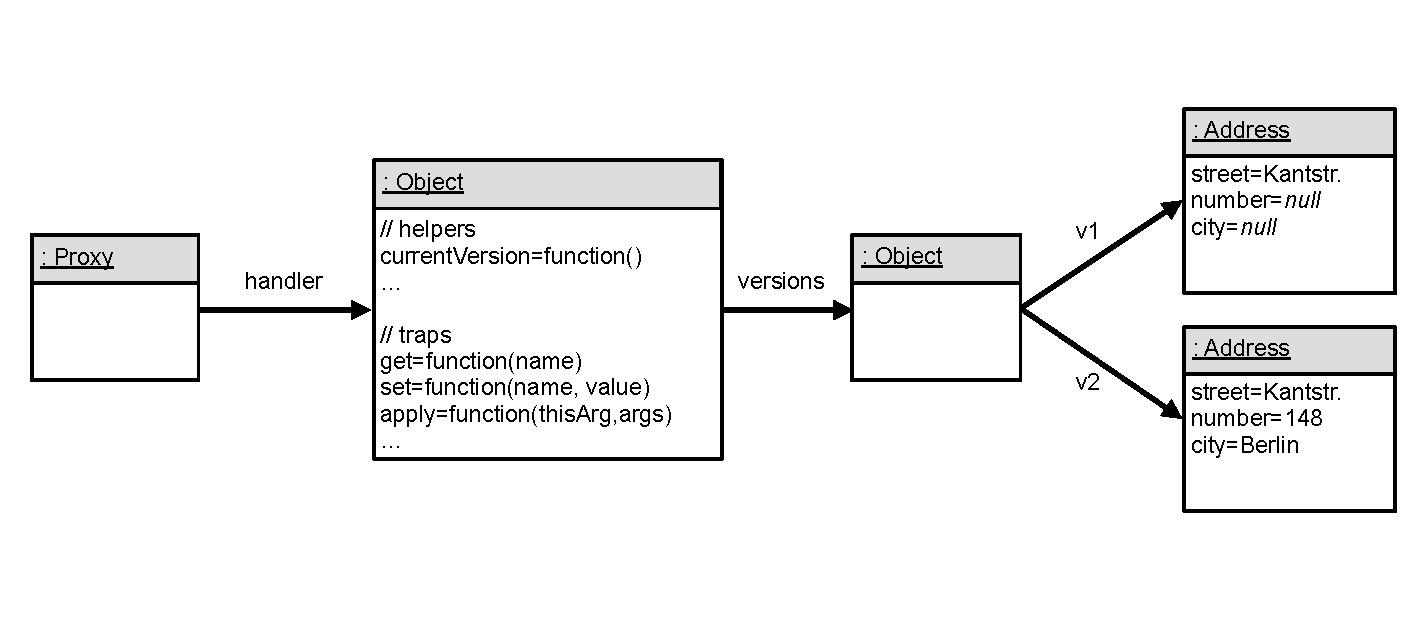
\includegraphics[width=\columnwidth]{figures/5_implementation/2_versioningProxy.pdf}
    \caption{A proxy with a handler that forwards to two versions of an \lstinline{address} object.}
    \label{fig:VersioningProxy}
\end{figure}

Our handler uses all available traps to forward to the current version of an object.
Each trap retrieves the current version of the object using the \lstinline{currentVersion} function, which selects the object version based on the active system version information.
The version information is available globally as \lstinline{lively.CurrentVersion}, an ordinary JavaScript object with three properties: an \lstinline{ID}, a \lstinline{predecessor}, and a \lstinline{successor}.

\begin{code}
currentVersion: function() {
    var objectVersion, systemVersion = lively.CurrentVersion;

    while(!objectVersion && systemVersion) {
        objectVersion = this.versions[systemVersion.ID];
        systemVersion = systemVersion.predecessor;
    }    
    return objectVersion;
}
\end{code}

All traps that intercept read-only access select the version to forward to using the \lstinline{currentVersion} function.
However, traps that intercept changes instead ensure a version of the object exists for the current system version, because the past cannot be allowed to change.
If no current version exists, the latest available version is copied and added to the \lstinline{versions} dictionary.
The traps that act in this way are \lstinline{set}, \lstinline{defineProperty}, \lstinline{deleteProperty}, \lstinline{freeze}, \lstinline{seal}, \lstinline{preventExtensions}, and \lstinline{apply}.
The \lstinline{apply} trap is included in this list because certain array functions such as \lstinline{push} and \lstinline{pop} are mutating, so when they are applied, a current version must be created.

The current version remains unchanged as long as the global \lstinline{lively.CurrentVersion} remains constant.
Changing the global version is an \emph{undo}, \emph{redo}, or \emph{commit} depending on whether the version is set to a previous, following, or new version.
The system provides convenience functions for these actions.
Using a global version of the system is reasonable as JavaScript is executed single-threaded, so the global version cannot be changed by another script.

\paragraph{Scope of the Versioning} \label{subsubsec:IMPLEMENTATION:5.2.1}
Using proxies allows multiple versions of most JavaScript objects, but certain objects represent the elements of the browser's \ac{dom} cannot be versioned with our implementation.
\ac{dom} objects are referred to from the browser's internal \ac{dom} structure, which is external to the JavaScript runtime.
In the Lively Kernel, this does not represent a problem, because the state of the \ac{dom} can be derived from morphs.
Whenever the system version changes, we update the \ac{dom} from the current set of visible morphs.

\subsection{Accessing All Mutable JavaScript Objects Through Proxies}

To be able to re-establish the system state with our versioning, we change the return values of all expressions that create new objects, arrays, and functions.
All these are mutable in JavaScript and might have arbitrary properties added to them.
Instead of letting these expressions return references to the new objects, the expressions return references to proxies for the objects.

In JavaScript, there are three categories of expressions that create new objects: 
\begin{itemize}
    \item literals, \eg\lstinline|{age: 12}|
    \item constructors, \eg\lstinline|new Person(12)|
    \item some built-ins, \eg\lstinline|Object.create(prototype, {age: 12})|
\end{itemize}

Our implementation uses source transformations and the proxy traps to have these expression return proxies.

\subsubsection{Transforming Literal Expressions}

We use source transformations to wrap literal expressions into calls to a \lstinline{proxyFor} function.
The expression \lstinline|{age: 12}| becomes \lstinline|proxyFor({age: 12})|, \lstinline{[a, b]} becomes \lstinline{proxyFor([a, b])}, and so forth.
However, some literal forms cannot be wrapped into function calls without introducing problems.
In particular, function declarations and accessor functions need to be handled differently.

\subsubsection{Function Declarations}

A \emph{function declaration} is a function literal that creates a named function and makes it available by the name in the surrounding scope:
\begin{code}
function add(a, b) { return a + b }
\end{code}

In contrast, a \emph{function expression} creates a function that needs to be assigned to a variable to be accessible:
\begin{code}
var add = function add(a, b) { return a + b }
\end{code}

Function expressions can create anonymous and named functions.
The previous example creates a named function.
Omitting the function name after the \lstinline{function} keyword would create an anonymous function.
While an anonymous function is always a function expression, a named function is either a function expression or a function declaration, depending on where it is expressed.
A function declaration cannot be nested into other statements such as variable assignments.

When a function declaration is wrapped into a \lstinline{proxyFor} function call, it becomes a function expression, meaning that it is no longer available by name in its surrounding scope.
After wrapping function declarations, they are assigned to matching variable names:
\lstinline|function div() {}| becomes \lstinline|var div = proxyFor(function div() {})|.
In addition, because function declarations get hoisted in JavaScript, transformed function declarations are moved to the beginning of the defining scope.

\subsubsection{Accessor Functions}

Accessor functions are functions that are executed instead of property reads or writes.
The following example uses an accessor function to allow reading a \lstinline{person}'s \lstinline{age} property, and have it calculated on access.

\begin{code}
var person = {
    birthdate: new Date(1984,27,5),
    get age() {
        return ageToday(this.birthdate);
    }
}
\end{code}

Wrapping the accessor function into a call to \lstinline{proxyFor} would not yield valid JavaScript syntax.
For this reason, the object is first created without the accessor function and the function is added afterwards using \lstinline{Object.defineProperty}.
The object literal and the call to \lstinline{Object.defineProperty} are wrapped into an anonymous functions that is immediately called to avoid polluting the variable bindings of the originally surrounding scope:

\begin{code}
var person = function() {
    var newObject = lively.proxyFor({
        birthdate: new Date(1984,27,5);
    });
    Object.defineProperty(newObject, "age", {
        get: lively.proxyFor(function age() {
            return ageToday(this.birthdate);
        })
        enumerable: true,
        configurable: true
    });
    return newObject;
}();
\end{code}

\subsection{Returning Proxies from Constructor Functions} 

In JavaScript, all functions can be used as constructors when called with the \lstinline{new} operator and if so used, they need to return proxies.
We use the \lstinline{construct} trap to simulate the object construction and return a proxy around the newly created object:
\begin{code}
construct: function(dummyTarget, args) {
        // find the current version of the constructor
    var constructor = this.currentVersion(),
        prototype = constructor.prototype || {},
        // create the object with the appropriate prototype
        newObject = Object.create(prototype),
        // call the constructor function
        result = constructor.apply(newObject, args);
    // return a proxy for the return value of the constructor
    // if any, otherwise for the new object
    return proxyFor(result || newObject);
}
\end{code}

% \begin{enumerate}
%     \item It retrieves the current version of the constructor (Line~1).
%     \item It creates a new object with the correct prototype (Line~2).
%     \item It calls the constructor with the new object as argument (Line~3).
%     \item It returns a proxy for return value of the constructor function or, if the constructor returned a falsy value, the new object (Line~4).
% \end{enumerate}

This way, all proxied functions return proxies when used as constructors.
With the previously presented transformations of literal expressions all literal functions are accessed through proxies.
Additionally, functions built into the JavaScript \acp{vm} are not created from function literals and must be wrapped separately.

\subsection{Wrapping Built-in Functions Into Proxies}

Some built-in functions can be used to create new objects.
For example, the built-in constructors \lstinline{Object} and \lstinline{Array} can be used to create new objects and arrays.
They return new objects when called with the \lstinline{new} operator and when called without.\\
Other global functions that create new objects include, for example, \lstinline{Object.create} and \lstinline{eval}.
The \lstinline{Object.create} function takes an object as argument, uses the argument as prototype of a new object, and returns the new object.
The \lstinline{eval} function takes a string as argument.
It evaluates the string as JavaScript code and, depending on the code string, can return new objects and even object graphs.


\subsubsection{Wrapping Built-in Constructor Functions}

We transform the built-in constructor functions by wrapping each into calls to the \lstinline{proxyFor} function.
\autoref{table:transformingBuiltInConstructors} shows this with two examples for the global \lstinline{Object} function.

\begin{table}[h]
\begin{center}
\begin{tabular}{| l | l | l |}
\hline
Input & Output \\ \hline
\lstinline|Object()| & \lstinline|proxyFor(Object)()| \\ \hline
\lstinline|new Object()| & \lstinline|new proxyFor(Object)()| \\ \hline
\end{tabular}
\end{center}
\caption[Table caption text]{Transforming built-in constructors.}
\label{table:transformingBuiltInConstructors}
\end{table}

The global symbols that are wrapped into calls to the \lstinline{proxyFor} are: \lstinline{Array}, \lstinline{Boolean}, \lstinline{Date}, \lstinline{Function}, \lstinline{Iterator}, \lstinline{Number}, \lstinline{Object}, \lstinline{RegExp}, \lstinline{String}, \lstinline{JSON}, \lstinline{Math}, \lstinline{Intl}, \lstinline{XMLHttpRequest}, \lstinline{Worker}, \lstinline{XMLSerializer}, \lstinline{window}, and \lstinline{document}.

Therefore, when these function objects are used as constructors, the \lstinline{construct} trap is called and returns proxies for the new objects as explained previously.
As these functions also create objects when called without the \lstinline{new} operator, we also have the \lstinline{apply} trap return proxies.
Therefore, the last line of our \lstinline{apply} trap is:
\iffalse
\begin{verbatim}\fi
\begin{code}
this.ensureProxied(result);
\end{code}
\iffalse
\end{verbatim}\fi

When the argument to the \lstinline{ensureProxied} function is already a proxy or an immutable value such as a string or a number, it returns the argument unchanged.
When the argument is, however, an object, an array, or a function, the \lstinline{ensureProxied} returns a proxy for that object.
This distinction is necessary as the \lstinline{apply} trap is called for all functions, not only built-in constructors.


\paragraph{Proxy Table}
With our solution each occurrence of a built-in constructor is wrapped into a separate call to the \lstinline{proxyFor} function.
Therefore, the same function objects are passed to the \lstinline{proxyFor} function multiple times.
To nevertheless return the same proxies for the same objects, we use a map to associate objects with their proxies.
This \emph{Proxy Table} is a weak-key map.
It does not prevent the garbage collector from reclaiming the objects used as keys.\\
Using the same proxies for the same objects is not only an optimization, but necessary for identity checks.
As a result of using the Proxy Table, the following statement returns \lstinline{true} for an arbitrary \lstinline{obj} object:
\iffalse
\begin{verbatim}\fi
\begin{code}
proxyFor(obj) === proxyFor(obj);
\end{code}
\iffalse
\end{verbatim}\fi



\subsubsection{Wrapping Other Built-In Functions}

Besides the built-in constructors, other built-in functions that create new objects need to return proxies as well.
For example, the following statement needs to return a proxy:
\iffalse
\begin{verbatim}\fi
\begin{code}
Object.create(proto);
\end{code}
\iffalse
\end{verbatim}\fi

In addition to the \lstinline{construct} trap and the \lstinline{apply} trap, we also have the \lstinline{get} trap return proxies.
Analogous to our \lstinline{apply} trap, the last line of our \lstinline{get} trap is:
\iffalse
\begin{verbatim}\fi
\begin{code}
this.ensureProxied(result);
\end{code}
\iffalse
\end{verbatim}\fi

Therefore, proxies for objects always return proxies when properties are read.
As a result, when the built-in constructor \lstinline{Object} gets wrapped into a call to the \lstinline{proxyFor} function as with the previously presented transformations, reading its \lstinline{create} property returns a proxy for the property.
Furthermore, this proxy's \lstinline{construct} trap returns a proxy when applied.
Thus, the following statement returns a proxy for the new object:
\iffalse
\begin{verbatim}\fi
\begin{code}
proxyFor(Object).create(proto);
\end{code}
\iffalse
\end{verbatim}\fi

Therefore, the previous transformations are sufficient to have all functions of the globals return proxies.

The \lstinline{eval} function, however, is handled differently.
It can return object graphs for the string argument provided.
For example, the following statement returns an object with an \lstinline{address} property, which is in turn an object:
\iffalse
\begin{verbatim}\fi
\begin{code}
eval("{age: 12, address: {street: 'Kantstr', city: 'Berlin'}}")
\end{code}
\iffalse
\end{verbatim}\fi

Therefore, it is not sufficient to ensure that the return value of the \lstinline{eval} function is a proxy.
Instead, the object in the example also needs to access its \lstinline{address} property via a proxy.\\
Moreover, the code passed to \lstinline{eval} could access built-in constructors or itself use the \lstinline{eval} function.
For this reason, we pass the string argument of the \lstinline{eval} function to our source transformations before it is evaluated.

The built-in functions could be overwritten globally to return proxies for the new objects, but our implementation of object versioning is a JavaScript library and makes itself use of the built-in types.
Additionally, at the time of writing, some JavaScript engines do not allow to overwrite particular built-in globals and we want our implementation of object versioning to work in every JavaScript engine that supports the ECMAScript 6 proxies.

\subsubsection{Implementation of Source Transformations}

Our implementation uses the \emph{UglifyJS}\footnote{\url{http://github.com/mishoo/UglifyJS2}, accessed March 12, 2014} library for all source transformations.
UglifyJS parses source code without relying on JavaScript exceptions.
Therefore, when code is transformed, it does not yield exceptions that could be caught by an open debugger.\\
In addition, UglifyJS supports Source Maps\footnote{\url{https://docs.google.com/document/d/1U1RGAehQwRypUTovF1KRlpiOFze0b-_2gc6fAH0KY0k/edit\#heading=h.ue4jskhddao6}, accessed May 2, 2014}.
This allows the browser's developer tools to present the original sources, even though transformed code is executed.





\subsection{Workarounds for the Current State of the ECMAScript 6 Proxies} \label{sec:IMPLEMENTATION:4}

Certain workarounds are required due to the preliminary implementation of ECMAScript 6 proxies in the JavaScript engines.

\paragraph{ECMAScript 6 Specification}
ECMAScript 6 will be the next version of JavaScript.
Its specification has not yet been finalized.
Drafts of it are released continuously with a target release date of December 2014\footnote{http://github.com/rwaldron/tc39-notes/blob/48c5d285bf8bf0c4e6e8bb0c02a7c840c01cd2ff/es6/2013-03/mar-13.md\#416-current-status-of-es6, accessed May 12, 2014}.
The current draft is Revision 24~\cite{Ecma2014ES6}.
It includes the proposal of the proxies we used for our implementation.

\paragraph{ECMAScript 6 Implementation}
The JavaScript engines used by Chrome and Firefox provide preliminary implementations for some of ECMAScript~6's features.
Among other features, they implement two different deprecated proposals of the proxy \ac{api}.
The \emph{harmony-reflect} library\footnote{\url{http://github.com/tvcutsem/harmony-reflect}, accessed February 3, 2014, used version 0.0.11} provides the current \ac{api} on top of these.
Our implementation uses the \emph{harmony-reflect} library and, therefore, works in Chrome and Firefox.

However, even with the library, three issues need to be addressed with technical workarounds:

\begin{enumerate}
    \item The proxies have to be provided with a target object, even when implementing virtual objects, and consistency invariants compare return values of the traps to the state of the target. 
    \item The proxies do not intercept the \lstinline{instanceof} operator, but always delegate to the current target.
    \item Certain built-in JavaScript functions don not handle proxies correctly.
\end{enumerate}

These workarounds might no longer be necessary once the ECMAScript 6 specification gets released and fully implemented by the JavaScript engines. 


\subsection{Disabling Target Object Invariants}

\subsubsection{Problem}
Even though the current ECMAScript 6 draft says otherwise\footnote{\url{http://people.mozilla.org/~jorendorff/es6-draft.html\#sec-proxy-object-internal-methods-and-internal-slots}, accessed April 15, 2014}, the proxies require a target object, as explained in Section~\label{subsec:IMPLEMENTATION:1.1}.
Even when the proxies are used as \emph{virtual objects}, they still are connected to a particular object.
Furthermore, the proxies are designed to ensure invariants between the return values of traps and the target's state~\cite{Cutsem2013TRP}.
For example, when an object's properties are made immutable through the \lstinline{Object.freeze} function, invariants ensure that the target object has in fact been frozen, even if the trap delegates the operation to another object.
Another invariant ensures that immutable values of the target object are reported by the traps.
Therefore, the \emph{get}-trap has to report the values of the target object when it previously has been frozen.
As a result, in our case, configuring any property as immutable would effectively make that property immutable for all versions.
Moreover, reading the property from object versions would potentially raise inconsistency errors.

\subsubsection{Solution}
For this reason, we adapted our copy of the \emph{harmony-reflect} library.
In particular, the \lstinline{Proxy} constructor takes a third argument.
This argument is a boolean that indicates whether a proxy is standing in for one target object or is a virtual object.
Providing \lstinline{true} as this argument effectively disables all consistency checks.


\subsubsection{Discussion}

Even with disabled consistency checks, the proxies still require actual objects as \emph{target} objects.
All trapped interactions are forwarded to the correct object versions, yet interactions that are not intercepted by any traps are still forwarded to the target objects.
The current draft does not include traps for the \lstinline{typeof} operator and the \lstinline{instanceof} operator.

The \lstinline{typeof} operator returns a certain set of values for different types.
Proxies stand in for objects, arrays, and functions.
It returns \emph{``object''} for arrays and objects and \emph{``function''} for functions.
Therefore, the target object of our proxies is an object when a proxy stands in for the versions of an array or an object, while it is a function when a proxy stands for the versions of functions.
Using a function object as target for a proxy that stands in for the version of a function is also necessary as the \lstinline{apply} and \lstinline{construct} traps are only called for proxies with function targets.

The \lstinline{instanceof} operator needs to be handled differently as it does not necessarily return the same value for all versions of an object.


\subsection{Forwarding the \emph{Instanceof} Operator}

\subsubsection{Problem}

The \lstinline{instanceof} operator can be used to test whether an object has a specific type.
In particular, it checks whether the \lstinline{prototype} property of a function is in an object's prototype chain.
For example, the following statement checks this for the \lstinline{Person} function and the \lstinline{me} object:
\iffalse
\begin{verbatim}\fi
\begin{code}
me instanceof Person
\end{code}
\iffalse
\end{verbatim}\fi

The prototype of an object is a property and can be changed at runtime.
Moreover, the \lstinline{prototype} property of a function is also mutable.
As any other property, these properties can be different in different object versions.
Thus, the \lstinline{instanceof} operator needs to be delegated to the current object version.
However, while trapping the \lstinline{instanceof} operator is under discussion\footnote{\url{http://wiki.ecmascript.org/doku.php?id=harmony:direct_proxies\#discussed_during_tc39_july_2012_meeting_microsoft_redmond}, accessed May 1, 2014}, there is currently no \lstinline{instanceof} trap.

\subsubsection{Solution}

Our implementation provides a custom \lstinline{Object.instanceof} function, which implements the semantics of the \lstinline{instanceof} operator but delegates to object versions when applied with a proxy as argument.
Consequentely, all usage of the \lstinline{instanceof} operator is transformed to the \lstinline{Object.instanceof} function.
\autoref{table:transformingInstanceof} shows this transformation by example.

\begin{table}[h]
\begin{center}
\begin{tabular}{| l | l | l |}
\hline
Input & Output \\ \hline
\lstinline|me instanceof Person| & \lstinline|Object.instanceof(me, Person)| \\ \hline
\end{tabular}
\end{center}
\caption[Table caption text]{Transforming the \lstinline{instanceof} operator.}
\label{table:transformingInstanceof}
\end{table}



\subsection{Unwrapping Versions for Native Code} \label{subsec:IMPLEMENTATION:4.3}


\subsubsection{Problem}

Some built-in JavaScript functions do not work correctly with proxies.
The functions react with errors, return wrong results, or silently ignore calls when applied with proxies as arguments or as their \lstinline{this}-context.
These built-in functions include, for example, the \lstinline{concat} function of array instances and all functions that manipulate the browser's \ac{dom}.
Moreover, string instance methods return wrong results when called with proxies for \lstinline{RegExp} arguments.

Furthermore, the \lstinline{onreadystatechanged} property of \lstinline{XMLHttpRequest} objects is not allowed to be proxy.
The \lstinline{onreadystatechanged} property is expected to be a function, which is called when the server responds to asynchronous \ac{http} requests. 
However, when a proxy is assigned as the property, the callback is not called with the response.


\subsubsection{Solution}

The problematic functions need to be provided with actual objects instead of proxies.
Therefore, our implementation retrieves the current object versions from the proxies and provides these to the functions.
The \lstinline{apply} trap unwraps all arguments and the \emph{thisContext} before applying built-in functions.

The \lstinline{apply} trap detects built-in functions through their print strings.
Built-in functions print to \emph{``[native code]''}, while functions created from literals print to their function body.\\
However, the \lstinline{apply} trap does not unwrap the arguments to specific built-in functions.
For example, the argument to an array's \lstinline{indexOf} function is not unwrapped as the function compares the argument's identity to the identity of array elements.
Additionally, the iterator functions of arrays handle proxies correctly.

Instances of strings are immutable and are not accessed through proxies in our implemention.
Therefore, unwrapping arguments in the \lstinline{apply} trap is not a solution for the string methods that do not handle proxies correctly.
For this reason, our implementation patches these string functions explicitly.
The functions are patched with functions that unwrap proxies before executing the original functions, as shown in \autoref{lst:stringPatch}.

\iffalse
\begin{verbatim}\fi
\begin{code}
var originalStringMatch = String.prototype.match;
String.prototype.match = function match(regexp) {
    var exp = Object.isProxy(regexp) ?
        regexp.proxyTarget() : regexp;
    return originalStringMatch.call(this, exp);
};
\end{code}
\iffalse
\end{verbatim}\fi

The four string methods that are patched in this way are: \lstinline{match}, \lstinline{search}, \lstinline{replace}, \lstinline{split}.

For the \lstinline{onreadystatechanged} property of \lstinline{XMLHttpRequest} objects, we have the \lstinline{set} trap unwrap the assigned proxy.
However, unwrapping a particular version of the callback function is potentially problematic.
Even though JavaScript does get executed with a single thread using cooperative scheduling, other scripts might get executed while the browser waits for the server's response.
Such concurrently executed scripts can switch the global version before the callback is called.
In a different version, the properties of the callback function can be different.
Moreover, the callback function might not be available in a previous version. 
Switching the system version while the browser waits for a response is a problem for which our implementation currently does not provide a workaround.


\subsection{Limitations of the Implementation}

We are aware of three limitations of our implementation.

\paragraph{Availability of ECMAScript 6 Proxies}
Our implementation requires the ECMAScript 6 proxies to be available.
The proxies are part of the next version of ECMAScript, which has currently neither been finalized nor completely implemented, as described in \autoref{sec:IMPLEMENTATION:4}.
For this reason, our implementation works only in versions of Firefox and Chrome that already implement preliminary versions of the proxies.
Furthermore, Chrome users need to enable the proxies explicitly\footnote{\url{http://plus.google.com/+PaulIrish/posts/T615Md5JPQG}, accessed May 13, 2014}.

\paragraph{Proxies Impede Developer Tools}
The current implementation of ECMAScript 6 proxies impedes debugging.
The proxies are partly implemented by a JavaScript library and every trapped object interaction is visible in multiple frames in the debugger.
Consequentely, the stack of the debugger is cluttered with frames that belong to the proxy implementation, not to application code.\\
Moreover, the developer tools in Chrome do not handle proxies correctly under all circumstances.
In particular, hovering over variable names that are bound to proxies yields errors.
It is also not possible to step into proxied functions in Chrome's debugger.
We did not test the developer tools of Firefox.

\paragraph{Concurrent JavaScript}
Even though JavaScript is executed with a single thread, scripts can be executed concurrently.
In general, scripts can be started from events and from other scripts using the \lstinline{setTimeout} or the \lstinline{setInterval} function.
Switching the system version can be problematic for such concurrently running scripts.\\
In the Lively Kernel, the \lstinline{setInterval} function is used to repeatedly execute a method of an object.
Re-establishing a previous version of the system can interfere with such ticking behavior.
For example, the method that is called repeatedly can be unavailable in the previous version.
For this reason, we stop scripts from future versions, when the system version changes.
However, we did not succeed in finding a way to restart the scripts again when the future versions are re-established.
Thus, subsequentely undoing and redoing changes can stop concurrently running scripts.

%%% Local Variables:
%%% mode: latex
%%% TeX-master: "../main"
%%% End:
